\documentclass{article}
\usepackage[utf8]{inputenc}
\usepackage{array}
\usepackage{classeRapport}
\usepackage{enumitem}
\usepackage{times}
\usepackage{graphicx,amsmath,amssymb, xcolor}
\usepackage[ruled,vlined, french]{algorithm2e}

    \SetKwInput{Declaration}{Declaration}
    \SetKw{KwA}{a}
    \SetKw{Retour}{retourner}
    \SetKwBlock{Deb}{debut}{fin}
    \SetKwIF{Si}{SinonSi}{Sinon}{si}{alors}{sinon si}{sinon}{finsi}
    \SetKwFor{Tq}{tant que}{faire}{finTantQue}
    \SetKwFor{Pour}{pour}{faire}{finPour}
    \SetKwRepeat{Repeter}{repeter}{jusqu’a}
    \SetKw{Pre}{Precondition(s)}

\usepackage{listings}
    \definecolor{darkWhite}{rgb}{0.94,0.94,0.94}
 
    \lstset{
      aboveskip=3mm,
      belowskip=-2mm,
      backgroundcolor=\color{darkWhite},
      basicstyle=\footnotesize,
      breakatwhitespace=false,
      breaklines=true,
      captionpos=b,
      commentstyle=\color{red},
      deletekeywords={...},
      escapeinside={\%*}{*)},
      extendedchars=true,
      framexleftmargin=16pt,
      framextopmargin=3pt,
      framexbottommargin=6pt,
      frame=tb,
      keepspaces=true,
      keywordstyle=\color{blue},
      language=C,
      literate=
      {²}{{\textsuperscript{2}}}1
      {⁴}{{\textsuperscript{4}}}1
      {⁶}{{\textsuperscript{6}}}1
      {⁸}{{\textsuperscript{8}}}1
      {€}{{\euro{}}}1
      {é}{{\'e}}1
      {è}{{\`{e}}}1
      {ê}{{\^{e}}}1
      {ë}{{\¨{e}}}1
      {É}{{\'{E}}}1
      {Ê}{{\^{E}}}1
      {û}{{\^{u}}}1
      {ù}{{\`{u}}}1
      {â}{{\^{a}}}1
      {à}{{\`{a}}}1
      {á}{{\'{a}}}1
      {ã}{{\~{a}}}1
      {Á}{{\'{A}}}1
      {Â}{{\^{A}}}1
      {Ã}{{\~{A}}}1
      {ç}{{\c{c}}}1
      {Ç}{{\c{C}}}1
      {õ}{{\~{o}}}1
      {ó}{{\'{o}}}1
      {ô}{{\^{o}}}1
      {Õ}{{\~{O}}}1
      {Ó}{{\'{O}}}1
      {Ô}{{\^{O}}}1
      {î}{{\^{i}}}1
      {Î}{{\^{I}}}1
      {í}{{\'{i}}}1
      {Í}{{\~{Í}}}1,
      morekeywords={*,...},
      numbers=left,
      numbersep=10pt,
      numberstyle=\tiny\color{black},
      rulecolor=\color{black},
      showspaces=false,
      showstringspaces=false,
      showtabs=false,
      stepnumber=1,
      stringstyle=\color{gray},
      tabsize=4,
      title=\lstname,
    }
\lstset{
  literate=
  {á}{{\'a}}1 {é}{{\'e}}1 {í}{{\'i}}1 {ó}{{\'o}}1 {ú}{{\'u}}1
  {Á}{{\'A}}1 {É}{{\'E}}1 {Í}{{\'I}}1 {Ó}{{\'O}}1 {Ú}{{\'U}}1
  {à}{{\`a}}1 {è}{{\`e}}1 {ì}{{\`i}}1 {ò}{{\`o}}1 {ù}{{\`u}}1
  {À}{{\`A}}1 {È}{{\'E}}1 {Ì}{{\`I}}1 {Ò}{{\`O}}1 {Ù}{{\`U}}1
  {ä}{{\"a}}1 {ë}{{\"e}}1 {ï}{{\"i}}1 {ö}{{\"o}}1 {ü}{{\"u}}1
  {Ä}{{\"A}}1 {Ë}{{\"E}}1 {Ï}{{\"I}}1 {Ö}{{\"O}}1 {Ü}{{\"U}}1
  {â}{{\^a}}1 {ê}{{\^e}}1 {î}{{\^i}}1 {ô}{{\^o}}1 {û}{{\^u}}1
  {Â}{{\^A}}1 {Ê}{{\^E}}1 {Î}{{\^I}}1 {Ô}{{\^O}}1 {Û}{{\^U}}1
  {œ}{{\oe}}1 {Œ}{{\OE}}1 {æ}{{\ae}}1 {Æ}{{\AE}}1 {ß}{{\ss}}1
  {ű}{{\H{u}}}1 {Ű}{{\H{U}}}1 {ő}{{\H{o}}}1 {Ő}{{\H{O}}}1
  {ç}{{\c c}}1 {Ç}{{\c C}}1 {ø}{{\o}}1 {å}{{\r a}}1 {Å}{{\r A}}1
  {€}{{\EUR}}1 {£}{{\pounds}}1
}
	
\begin{document}

\PageDeGarde	
{cover.jpeg} % image sur la page de garde
{Correcteur Orthographique} % titre principal
{Vous n'avez jamais aussi bien écrit !} % sous-titre
{Fatiha \textsc{Hammouche} \\
Florine \textsc{Chevrier} \\
Loïck \textsc{Toupin} \\
Noé \textsc{Tatoud}}
{Algo - ITI - 2021} % bas de page

\Page{INSALogo}{rien.png} % logo de bas de page (en bas a droite)

\tableofcontents

\clearpage
\section{Introduction}
Dans le cadre de nos études dans la filière ITI à l’INSA de Rouen, nous avons réalisé un projet d’algorithmie en C. Le but de ce projet était de réaliser un correcteur orthographique. Ce projet est le premier que nous avons eu à réaliser du début à la fin en autonomie presque complète. Cela nous a permis de faire face à de nombreuses difficultés et ainsi de progresser dans de divers domaines.
\newline
En effet, ce projet a évidemment sollicité nos connaissances algorithmiques, mais également notre capacité à travailler en groupe. Nous avons appris à nous organiser, mais aussi à mieux communiquer. Nous nous sommes adaptés aux autres, notamment en codant de façon claire et précise pour que nos collègues puissent comprendre ce que nous avions fait. Afin de faciliter la gestion de ce projet, nous devions utiliser Git dont nous nous étions déjà servi à d’autres occasions mais pour la plupart d’entre nous, nous ne le maîtrisions pas encore. L’utilisation de cette plateforme est donc une autre compétence essentielle que nous avons pu développer. Nous avons tous aussi progressé en C, qui est un langage que nous avons commencé à étudier au début de l’année, et nous avons appris à documenter notre code avec Doxygen. Nous avons également amélioré nos compétences en \LaTeX que nous avons utilisé pour la rédaction du rapport.
\newline
Nous présentons donc dans ce rapport le résultat de notre travail, en commençant par l’analyse, puis la conception préliminaire et enfin la conception détaillée.
\clearpage
\section{TAD}
	\documentclass{article}
\usepackage[utf8]{inputenc}
\usepackage{enumitem}
\usepackage{amssymb}
\usepackage[hmargin=2cm,vmargin=0cm]{geometry}
\begin{document}
    \noindent
    \textbf{Nom}: Mot \\
    \textbf{Utilise}: Chaine de caracteres,NaturelNonNul,Caractere,Booleen \\
    \textbf{Opérations}: \begin{itemize}[label=$\ $, leftmargin=2cm, itemsep=0cm]
        \item estUnMotValide: Chaine de caracteres $\rightarrow $ Booleen
        \item creerUnmot: ChaineDeCaracteres $ \rightarrow$ Mot
        \item longueur: Mot $ \rightarrow$  NaturelNonNul
        \item accederAuIemeCaractere: Mot $ \times $ NaturelNonNul $ \nrightarrow$  Caractere
        \item sontIdentiques Mot $ \times $ Mot $ \rightarrow$  Booléen
    \end{itemize}
    
    \textbf{Sémantique}: \begin{itemize}[label=$\- $, leftmargin=2cm, itemsep=0cm]
      \item creerUnMot:création d’un mot à partir d’une chaine de caractère.
        \item estUnMotValide: verifier si le mot est bien composé des lettres, renvoit VRAI si le mot contient que les lettres et renvoit FAUX sinon.
        \item longueur: donner la longueur d’un mot.
        \item accederAuIemeCaractere: accéder à un certain caractère d`un mot en precisant son indice.
         \item sontIdentiques : vérifier si deux mots sont identiques.
    \end{itemize}

    \textbf{Préconditions}: \begin{itemize}[label=$\- $, leftmargin=2cm, itemsep=0cm]
        \item accederAuIemeCaractere(mot, i) : 1 $\leq$ i $\leq$ longueur(mot)
    \end{itemize}
\end{document}

	\clearpage
	\documentclass{article}
\usepackage[utf8]{inputenc}
\usepackage{enumitem}
\usepackage{amssymb}
\usepackage[hmargin=2cm,vmargin=0cm]{geometry}
\begin{document}
    \noindent
    Nom: Dictionnaire \\
    Utilise: Mot,Mode,FichierTexte,Booleen \\
    Type Mode={Lecture,Ecriture} \\
    Opérations: \begin{itemize}[label=$\ $, leftmargin=2cm, itemsep=0cm]
        \item creerDictionnaire: FichierTexte $\rightarrow $ Dictionnaire
        \item contientMot: Dictionnaire $\times$ Mot $\rightarrow $ Booléen
        \item ajouterListeMots : Dictionnaire $\times$ FichierTexte $ \rightarrow$ Dictionnaire
        \item ouvrirDictionnaire : Dictionnaire $\times$ Mode $ \rightarrow$ Dictionnaire
        \item fermerDictionnaire : Dictionnaire $ \nrightarrow$ Dictionnaire
        \item estOuvert : Dictionnaire $ \rightarrow$ Booleen
        \item modeDictionnaire : Dictionnaire $ \nrightarrow$ Mode
        
        
    \end{itemize}
    
    Sémantique: \begin{itemize}[label=$\- $, leftmargin=2cm, itemsep=0cm]
        \item creerDictionnaire : création d’un dictionnaire à partir d’un fichierTexte (trie et crée l'arborescence)
        \item contientMot : renvoit VRAI si le mot est dans le dictionnaire, FAUX sinon
        \item ajouterListeMots: ajoute une liste de mots dans le dictionnaire,en les insérant dans l'aborescence, en écrasant si le mot est déjà présent
        \item ouvrirDictionnaire : ouvre le dictionnaire dans le mode choisi
        \item fermerDictionnaire : referme le dictionnaire ouvert
        \item estOuvert : renvoie le booléen correspondant à l'état ouvert ou fermé du dictionnaire
        \item modeDictionnaire : renvoie le mode du dictionnaire : Lecture ou Ecriture
    \end{itemize}

    Préconditions: \begin{itemize}[label=$\- $, leftmargin=2cm, itemsep=0cm]
        \item fermerDictionnaire : estOuvert(Dictionnaire)
        \item modeDictionnaire : estOuvert(Dictionnaire)
    \end{itemize}
\end{document}

	\clearpage
	\documentclass{article}
\usepackage[utf8]{inputenc}
\usepackage{enumitem}
\usepackage{amssymb}
\usepackage[hmargin=2cm,vmargin=0cm]{geometry}
\begin{document}
    \noindent
    \\
    \textbf{Nom}: CorrecteurOrthographique \\
    \textbf{Utilise}: \textbf{Mot, Dictionnaire, Ensemble$<$Mots$>$} \\
    \textbf{Opérations}: \begin{itemize}[label=$\ $, leftmargin=2cm, itemsep=0cm]
        \item correcteur : \textbf{Dictionnaire $\times$ Mot $\rightarrow$ CorrecteurOrthographique}
        \item obtenirMotACorriger : \textbf{CorrecteurOrthographique $\rightarrow$ Mot}
        \item obtenirDictionnaire : \textbf{CorrecteurOrthographique $\rightarrow$ Dictionnaire}
        \item obtenirCorrections : \textbf{CorrecteurOrthographique $\rightarrow$ Ensemble$<$Mots$>$}
        \item fixerDico : \textbf{CorrecteurOrthographique $\times$ Dictionnaire $\rightarrow$ CorrecteurOrthographique}
        \item fixerMotACorriger : \textbf{CorrecteurOrthographique $\times$ Mot $\rightarrow$ CorrecteurOrthographique}
        \item ajouterNouvellesCorrections : \\ \textbf{CorrecteurOrthographique $\times$ Ensemble$<$Mot$>$ $\rightarrow$ CorrecteurOrthographique}
        \item trouverCorrectionsPossibles : \textbf{CorrecteurOrthographique $\rightarrow$ CorrecteurOrthographique}
        \item remplacerIemeLettreEnBoucle : \textbf{Mot $\times$ Naturel $\rightarrow$ Ensemble$<$Mot$>$}
        \item strategieRemplacerLettres : \textbf{CorrecteurOrthographique $\rightarrow$ CorrecteurOrthographique}
        \item strategieSupprimerLettres : \textbf{CorrecteurOrthographique $\rightarrow$ CorrecteurOrthographique}
        \item strategieInverserDeuxLettresConsecutives : \textbf{CorrecteurOrthographique $\rightarrow$ CorrecteurOrthographique}
        \item insererIemeLettreEnBoucle : \textbf{Mot $\times$ Naturel $\rightarrow$ Ensemble$<$Mot$>$}
        \item strategieInsererLettres : \textbf{CorrecteurOrthographique $\rightarrow$ CorrecteurOrthographique}
        \item strategieDecomposerMot : \textbf{CorrecteurOrthographique $\rightarrow$ CorrecteurOrthographique}
    \end{itemize}
    \textbf{Sémantique}: \begin{itemize}[label=$\- $, leftmargin=2cm, itemsep=0cm]
        \item obtenirMotACorriger : Permet d'accèder au mot à corriger 
        \item obtenirDictionnaire : Permet d'accèder au dictionnaire 
        \item obtenirCorrections : Permet d'accèder aux corrections du mot
        \item fixerDico : Donne un dictionnaire à utiliser au correcteur.
        \item fixerMotACorriger : Donne un mot à corriger au correcteur.
        \item ajouterNouvellesCorrections : Ajoute de nouvelles corrections du mot à corriger au correcteur.
        \item trouverCorrectionsPossibles : Renvoie l'ensemble des corrections possibles du mot à corriger.
        \item remplacerIemeLettreEnBoucle : Remplace une lettre du mot par toutes les autres de l'alphabet, une par une
        \item strategieRemplacerLettres : Remplace toutes les lettres du mot par tous les caractères de l'alphabet tour à tour et ajoute les corrections valides au correcteur
        \item strategieSupprimerLettres : Supprime les lettres du mot tour à tour et ajoute les corrections valides au correcteur
        \item strategieInverserDeuxLettresConsecutives : Inverse les lettres du mot deux à deux, les unes après les autres et ajoute les corrections valides au correcteur
        \item remplacerIemeLettreEnBoucle : Insère toutes les lettres de l'alphabet une par une à un endroit du mot
        \item strategieInsererLettres : Insère un par un tous les caractères alphabétiques à tous les endroits du mot et ajoute les corrections valides au correcteur
        \item strategieDecomposerMot : Décompose le mot en deux parties de toutes les façons possibles et ajoute les corrections valides au correcteur
    \end{itemize}
        
    \textbf{Préconditions}: \begin{itemize}[label=$\- $, leftmargin=2cm, itemsep=0cm]
        \item correcteur(unDico, unMotFaux) : non(estUnMotDuDictionnaire(unDico, unMotFaux)
        \item fixerMotACorriger(unCorrecteur, unMotFaux) : \\non(estUnMotDuDictionnaire(obtenirDictionnaire(unCorrecteur), unMotFaux))
    \end{itemize}
        
\end{document}

	\clearpage
	
    \textbf{Type Mode} = \{lecture,ecriture\} \\
    \textbf{Nom}: FichierTexte \\
    \textbf{Utilise}: \textbf{Chaine de caracteres,Mode,Caractere,Booleen} \\
    \textbf{Opérations}: \begin{itemize}[label=$\ $, leftmargin=2cm, itemsep=0cm]
        \item fichierTexte: \textbf{Chaine de caracteres $\rightarrow $ FichierTexte}
        \item ouvrir: \textbf{FichierTexte $ \times $ Mode $ \nrightarrow$ Fichier}
        \item fermer: \textbf{FichierTexte$  \nrightarrow $ FichierTexte}
        \item estOuvert: \textbf{FichierTexte$ \nrightarrow$  Booleen}
        \item mode: \textbf{FichierTexte $\nrightarrow $ Mode}
        \item finFichier: \textbf{FichierTexte $ \nrightarrow $ Booleen}
        \item ecrireChaine: \textbf{FichierTexte $ \times $ Chaine $ \nrightarrow$  FichierTexte}
        \item lireChaine: \textbf{FichierTexte $ \nrightarrow$  FichierTexte $ \times $ Chaine}
        \item ecrireCaractere: \textbf{FichierTexte $ \times $ Caractere $ \nrightarrow$  FichierTexte}
        \item lireCaractere: \textbf{FichierTexte $ \nrightarrow$  FichierTexte $ \times $ Caractere}
    \end{itemize}
    
    \textbf{Sémantique}: \begin{itemize}[label=$\- $, leftmargin=2cm, itemsep=0cm]
        \item fichierTexte: création d’un fichier texte à partir d’un fichier identifié par son nom.
        \item ouvrir: ouvre un fichier texte en lecture ou écriture. Si le mode est écriture et que le fichier existe, alors ce dernier est écrasé.
        \item fermer: ferme un fichier texte.
        \item lireCaractere: lit un caractère à partir de la position courante du fichier.
        \item lireChaine: lit une chaîne (jusqu'à un retour à la ligne ou la fin de fichier) à partir de la position courante du fichier.
        \item ecrireCaractere: écrit un caractère à partir de la position courante du fichier.
        \item ecrireChaine: écrit une chaîne suivie d'un retour à la ligne à partir de la position courante du fichier.
    \end{itemize}

    \textbf{Préconditions}: \begin{itemize}[label=$\- $, leftmargin=2cm, itemsep=0cm]
        \item ouvrir(f): non(estOuvert(f))
        \item fermer(f): estOuvert(f)
        \item finFichier(f): mode(f)=lecture
        \item lireXX(f): estOuvert(f) et mode(f)=lecture et non finFichier(f)
        \item ecrireXX(f): estOuvert(f) et mode(f)=ecriture
    \end{itemize}



\clearpage
\section{Analyses Descendantes}
  \subsection{Analyse Descendante Générale}
  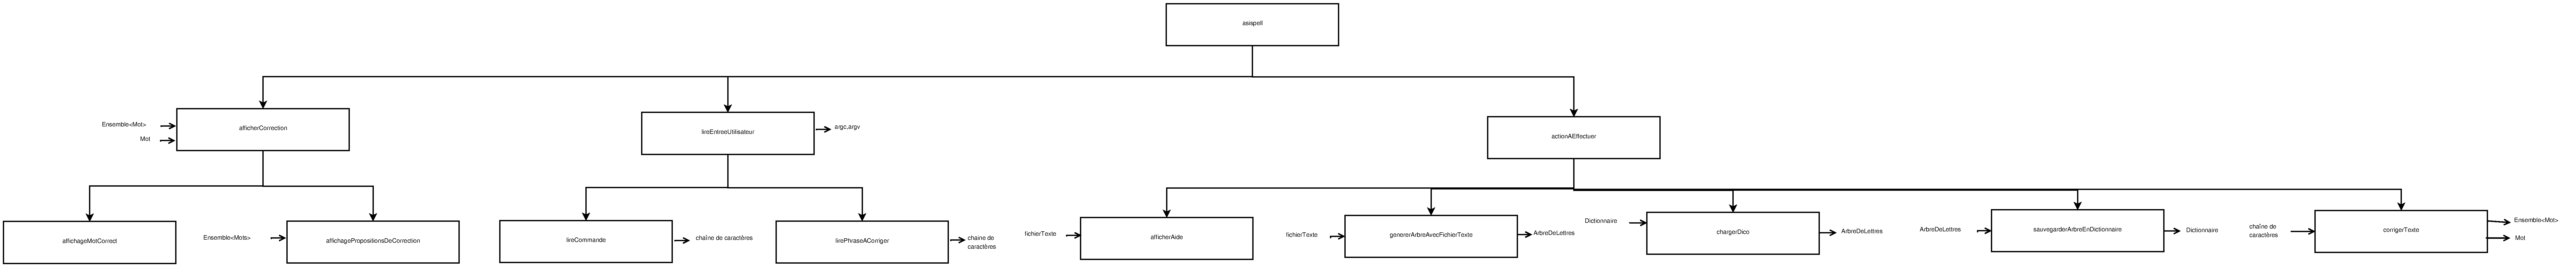
\includegraphics[width=1\textwidth]{AD/AnalyseDescendante.eps}
  \subsection{Analyse Descendante de corrigerTexte}
  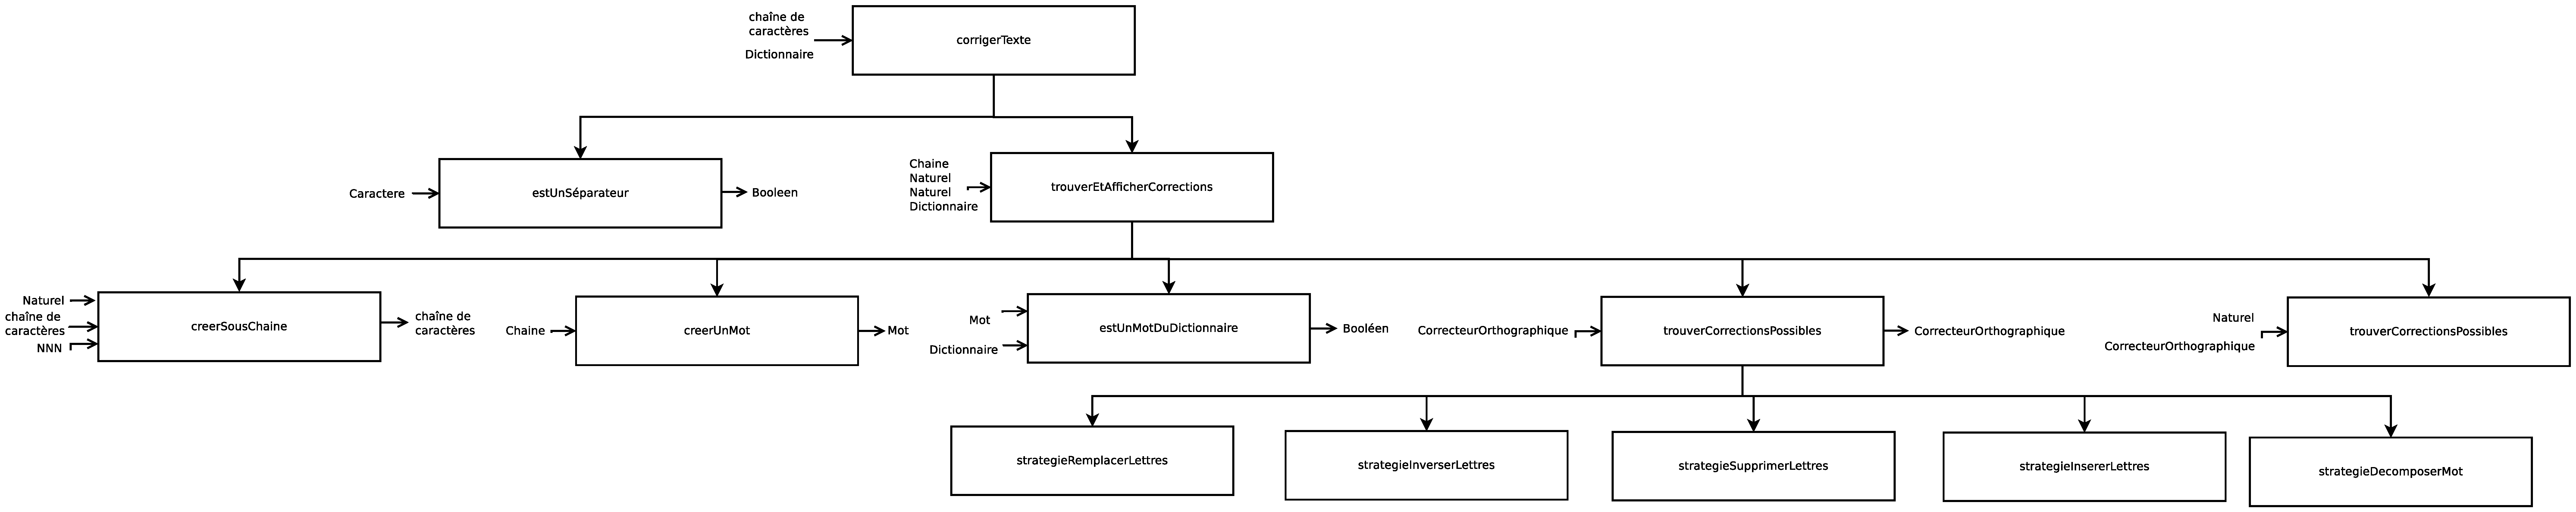
\includegraphics[width=1\textwidth]{AD/corrigerTexte.eps}
  \subsection{Analyse Descendante de genererDictionnaireAvecFichierTexte}
  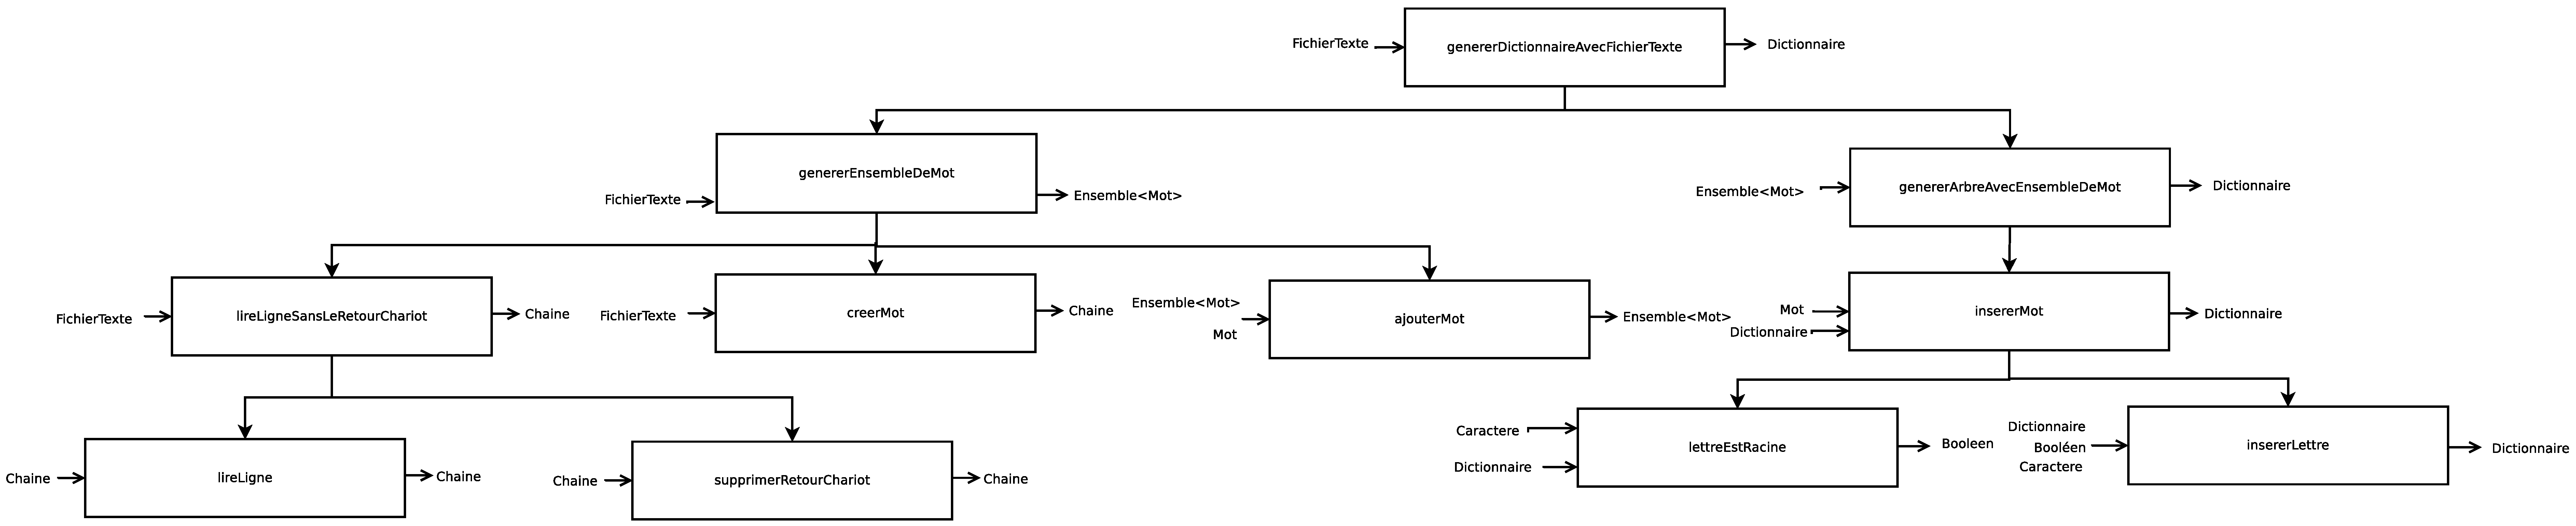
\includegraphics[width=1\textwidth]{AD/genererDictionnaireAvecFichierTexte.eps}

\clearpage
\section{Conception des TAD}
	
	\documentclass{article}
\usepackage[utf8]{inputenc}
\usepackage{enumitem}
\usepackage{amssymb}
\usepackage{times}
\usepackage{fancyhdr,graphicx,amsmath,amssymb}
\usepackage[ruled,vlined, french]{algorithm2e}
    \SetKwInput{Declaration}{Declaration}
    \SetKw{KwA}{a}
    \SetKw{Retour}{retourner}
    \SetKwBlock{Deb}{debut}{fin}
    \SetKwIF{Si}{SinonSi}{Sinon}{si}{alors}{sinon si}{sinon}{finsi}
    \SetKwFor{Tq}{tant que}{faire}{finTantQue}
    \SetKwFor{Pour}{pour}{faire}{finPour}
    \SetKwRepeat{Repeter}{repeter}{jusqu’a}
    \SetKw{Pre}{Precondition(s)}
\usepackage[hmargin=2cm,vmargin=0cm]{geometry}

\begin{document}
    \pagestyle{empty}
    \noindent

    \section*{Mot}
    \subsection*{Conception préliminaire}
    
    \subsubsection*{Signatures}

	\begin{itemize}[label=$\ $, leftmargin=1cm]
		 \item \textbf{fonction} estUnMotValide(uneChaine : Chaine de Caractère) :Booleen
		 \item \textbf{fonction} creerUnMot(uneChaine : Chaine de Caractère) : Mot
		 \item \textbf{fonction} longueur(unMot : Mot) : Naturel
		 \item \textbf{fonction} accederAuIemeCaractere(unMot : Mot, position : NaturelNonNul) : Caractere
		 \begin{itemize}[label=$| $]
            \item \textbf{précondition:} position $<$ longueur(unMot)
         \end{itemize}
         \item \textbf{fonction} sontEgaux(unMot, unAutreMot : Mot) : Booleen
	\end{itemize} 
    
\end{document}

	\clearpage

	\section*{Dictionnaire}
    \subsection*{Conception préliminaire}
    \subsubsection*{Signatures}

	\begin{itemize}[label=$\ $, leftmargin=1cm]
		 \item \textbf{fonction} genererArbreAvecEnsembleDeMot(lesMots : Ensemble$<$Mot$>$): ArbreDeLettres
		 \begin{itemize}[label=$| $] 
            \item \textbf{précondition:} non estVide(lesMots) 
         \end{itemize}
		 \item \textbf{fonction} estUnMotDuDictionnaire(unArbre : ArbreDeLettres, unMot : Mot):Booléen
         \item \textbf{fonction} chargerDico(unDictionnaire : Dictionnaire) :ArbreDeLettres 
         \item \textbf{fonction} sauvegarderArbreEnDictionnaire(unArbre : Arbre): Dictionnaire
	\end{itemize}
	
    \subsection*{Conception détaillée}

    \begin{function}
    \SetAlgoLined
    \caption{genererArbreAvecEnsembleDeMot (lesMots : Ensemble$<$Mot$>$): ArbreDeLettres}
    \Pre{non estVide(lesMots)} \\
    \Declaration{\\
        unArbre : ArbreDeLettres \\
        i : Entier
        }
    \Deb{
        \Pour{i $\gets$ 1 \textbf{allant à} longueur(lesMots)}
        {insererMotALaBonnePlace(unArbre, obtenirElement(lesMots, i))}
        \Retour{unArbre}
    }
    \end{function}
    
       \begin{function}
    \SetAlgoLined
    \caption{chargerDico(unDictionnaire : Dictionnaire) :ArbreDeLettres }
    \Declaration{\\
        }
    \Deb{
        \Retour{}
    }
    \end{function}
    
      \begin{function}
    \SetAlgoLined
    \caption{estUnMotDuDictionnaire(unArbre : ArbreDeLettres, unMot : Mot):Booléen}
    \Declaration{\\ temp : ArbreDeLettres
        }
    \Deb{
        \Si{longueur(unMot) = 1}
            {
            \Retour{non(estVide(unArbre) ou non(obtenirBooleen(unArbre))}
            }
        \Sinon
            {\Si{non estVide(unArbre)}
                {\Si{iemeCaractere(unMot,1) = obtenirLettre(unArbre)}
                    {
                    unMot $\gets$ supprimerIemeLettre(unMot, 1) \\
                    temp $\gets$ obtenirFilsGauche(unArbre)\\
                    \Retour{estUnMotDuDictionnaire(unMot, temp)}
                    }
                 \Sinon
                    {
                    temp $\gets$ obtenirFrere(unArbre)\\
                    \Retour{estUnMotDuDictionnaire(unMot, temp)}
                    }
                }
             \Sinon{\Retour{FAUX}}
            }
        
        }
    \end{function}
    
      \begin{function}
    \SetAlgoLined
    \caption{sauvegarderArbreEnDictionnaire(unArbre : Arbre): Dictionnaire}
    \Declaration{\\
        }
    \Deb{
        \Retour{}
    }
    \end{function}
	\clearpage

	\documentclass{article}
\usepackage[utf8]{inputenc}
\usepackage{enumitem}
\usepackage{amssymb}
\usepackage{times}
\usepackage{fancyhdr,graphicx,amsmath,amssymb}
\usepackage[ruled,vlined, french]{algorithm2e}
    \SetKwInput{Declaration}{Declaration}
    \SetKw{KwA}{a}
    \SetKw{Retour}{retourner}
    \SetKwBlock{Deb}{debut}{fin}
    \SetKwIF{Si}{SinonSi}{Sinon}{si}{alors}{sinon si}{sinon}{finsi}
    \SetKwFor{Tq}{tant que}{faire}{finTantQue}
    \SetKwFor{Pour}{pour}{faire}{finPour}
    \SetKwRepeat{Repeter}{repeter}{jusqu’a}
    \SetKw{Pre}{Precondition(s)}
\usepackage[hmargin=2cm,vmargin=0cm]{geometry}

\begin{document}
    \pagestyle{empty}
    \noindent
    Type Mot = Structure \\
    \textbf{chaine}: ChaineDeCaractere \\
    \textbf{longueur}: Naturel\\
    Fin Structure

    \section*{Correcteur Orthographique}
    \subsection*{Conception préliminaire}
   
    \subsubsection*{Signatures}

	\begin{itemize}[label=$\ $, leftmargin=1cm]
		 \item \textbf{procedure} remplacerIemeLettre(\textbf{E/S} mot : Mot, \textbf{E} c : Caractere, \textbf{E} i : Naturel)
		 \item \textbf{procedure} supprimerIemeLettre(\textbf{E/S} unMot : Mot, \textbf{E} position : Naturel)
		 \begin{itemize}[label=$| $]
            \item \textbf{précondition:} longueur(mot)$\ge$1 et i$\le$longueur
         \end{itemize}
		 \item \textbf{procedure} inverserDeuxLettresConsecutives(\textbf{E/S} unMot : Mot,  \textbf{E} i : NaturelNonNul)
		 \begin{itemize}[label=$| $]
            \item \textbf{précondition:} longueur(mot)$>$1 et i$\le$longueur
         \end{itemize}
		 
		 \item \textbf{procedure} insererLettre(\textbf{E/S} unMot : Mot, \textbf{E} i : Naturel, \textbf{E} c : Caractere)
		 \begin{itemize}[label=$| $]
            \item \textbf{précondition:} i$\le$ longueur(mot)
         \end{itemize}
         \item \textbf{fonction} decomposerMot(unMot : Mot, i : NaturelNonNul) : Mot, Mot
		 \begin{itemize}[label=$| $]
            \item \textbf{précondition:} i$\le$ longueur(mot)
         \end{itemize}
         \item \textbf{procedure} minuscule(\textbf{E/S} mot : Mot)
        
	\end{itemize} 
    
    \subsection*{Conception détaillée}

    \begin{procedure}
    \SetAlgoLined
    \caption{remplacerIemeLettre(\textbf{E/S} mot : Mot,\textbf{E} c : Caractere, \textbf{E} position : naturel)}
    \Declaration{}
    \Deb{
        supprimerIemeLettre(mot,position)\;
        insererLettre(mot,position,caractere)\;
    }
    \end{procedure}
    
    \begin{procedure}
    \SetAlgoLined
    \caption{supprimerIemeLettre(\textbf{E/S} unMot, \textbf{E} position : Naturel)}
    \Pre{longueur(mot)$\ge$1 et i$\le$longueur}\\
    \Declaration{}
    \Deb{
       ChaineDeCaractere.supprimerIemeLettre(unMot.chaine,position)\;
       unMot.longueur $\gets$ unMot.longueur-1 \;
    }
    \end{procedure}
    
    \begin{procedure}
    \SetAlgoLined
    \caption{inverserDeuxLettresConsecutives(\textbf{E/S} unMot : Mot, \textbf{E} i : NaturelNonNul)}
    \Pre{longueur(mot)$\ge$1 et i$\le$longueur}\\
    \Declaration{c1,c2 : Caractere}
    \Deb{
    	c1 $\gets$ Mot.accederAuIemeCaractere(unMot,i)\;
    	c2 $\gets$ Mot.accederAuIemeCaractere(unMot,i+1)\;
    	remplacerIemeLettre(unMot, c2, i)\;
    	remplacerIemeLettre(unMot, c1, i+1)\;
    }
    \end{procedure}
    
     \begin{procedure}
    \SetAlgoLined
    \caption{insererLettre(\textbf{E/S} unMot : Mot, \textbf{E} position : Naturel, c : Caractere)}
    \Pre{i$\le$ longueur(mot)}\\
    \Declaration{}
    \Deb{
       ChaineDeCaratere.insererLettre(unMot.chaine,position,c)\;
       unMot.longueur $\gets$ unMot.longueur + 1\;
    }
    \end{procedure}
    
    \begin{function}
    \SetAlgoLined
    \caption{decomposerMot(unMot : Mot, position : NaturelNonNul) : Mot, Mot}
    \Pre{i$\le$ longueur(mot)}\\
    \Declaration{mot1, mot2 : Mot, c : Caractere, chaine1, chaine2 : ChaineDeCaractere}
    \Deb{
    	mot1 $\gets$ creerUnMot("")\;
    	mot2 $\gets$ creerUnMot("")\;
       \Pour{i $\gets$ 1 à position-1}{
        	c $\gets$ Mot.accederAuIemeCaractere(unMot,i)\;
        	insererLettre(mot1, i, c);
        }
        \Pour{i $\gets$ position à unMot.longueur}{
        	c $\gets$ Mot.accederAuIemeCaractere(unMot,i)\;
        	insererLettre(mot2, i, c);
        }
      	\Retour{mot1, mot2}
    }
    \end{function}
 
\end{document}

	\clearpage

	
    \section*{FichierTexte}
    \subsection*{Conception préliminaire}
    \subsubsection*{Structure}

    Type FichierTexte = Structure
	\begin{itemize}[label=$\ $, leftmargin=2cm]
		 \item fichier : Fichier
		 \item mode : Mode
	\end{itemize}
    finStructure
    
    \subsubsection*{Signatures}

	\begin{itemize}[label=$\ $, leftmargin=1cm]
		 \item \textbf{fonction} fichierTexte(chaine : Chaine de Caractère):FichierTexte
		 \item \textbf{procédure} ouvrir(E/S fichier:FichierTexte,E mode : Mode)
		 \begin{itemize}[label=$| $]
            \item \textbf{précondition:} non estOuvert(f)
         \end{itemize}
         \item \textbf{procédure} fermer(E/S fichier:FichierTexte)
		 \begin{itemize}[label=$| $]
            \item \textbf{précondition:} estOuvert(f)
         \end{itemize}
		 \item \textbf{fonction} estOuvert(fichier:FichierTexte):Booleen
		 \item \textbf{fonction} mode(fichier:FichierTexte) : Mode
		 \item \textbf{fonction} finFichier(fichier:FichierTexte):Booleen
		 \begin{itemize}[label=$| $]
            \item \textbf{précondition:} mode(f)=lecture
         \end{itemize}
         \item \textbf{procédure} ecrireChaine(E/S fichier:FichierTexte, E chaine:Chaine de Caractère)
         \begin{itemize}[label=$| $]
            \item \textbf{précondition:} estOuvert(f) et mode(f)=ecriture
         \end{itemize}
         \item \textbf{procédure} lireChaine(E/S fichier:FichierTexte, S chaine:Chaine de Caractère)
         \begin{itemize}[label=$| $]
            \item \textbf{précondition:} estOuvert(f) et mode(f)=lecture et non finFichier(f)
         \end{itemize}
         \item \textbf{procédure} ecrireCaractere(E/S fichier:FichierTexte, E caractere:Caractère)
         \begin{itemize}[label=$| $]
            \item \textbf{précondition:} estOuvert(f) et mode(f)=ecriture
         \end{itemize}
         \item \textbf{procédure} lireCaractere(E/S fichier:FichierTexte, S caractere:Caractère)
         \begin{itemize}[label=$| $]
            \item \textbf{précondition:} estOuvert(f) et mode(f)=lecture et non finFichier(f)
         \end{itemize}

	\end{itemize} 
    
    \subsection*{Conception détaillée}




\clearpage
\section{Code C}

	\lstinputlisting[language=C]{../programme/src/ArbreDeLettres.c}	
	\lstinputlisting[language=C]{../programme/src/CorrecteurOrthographique.c}
	\lstinputlisting[language=C]{../programme/src/corrigerTexte.c}
	\lstinputlisting[language=C]{../programme/src/Dictionnaire.c}
	\lstinputlisting[language=C]{../programme/src/EnsembleDeMot.c}
	\lstinputlisting[language=C]{../programme/src/FichierTexte.c}
	\lstinputlisting[language=C]{../programme/src/ListeChaineeDeMot.c}
	\lstinputlisting[language=C]{../programme/src/main.c}
	\lstinputlisting[language=C]{../programme/src/Mot.c}

\clearpage
\section{Tests unitaires}
	\lstinputlisting[language=C]{../programme/src/testArbreDeLettres.c}
	\lstinputlisting[language=C]{../programme/src/testCO.c}
	\lstinputlisting[language=C]{../programme/src/testEDM.c}
	\lstinputlisting[language=C]{../programme/src/testLCDM.c}
	\lstinputlisting[language=C]{../programme/src/testMot.c}

\clearpage
\section{Organisation}
Du début à la fin de ce projet, nous nous sommes réparti le travail entre les différents TADs. De l'analyse aux tests, nous nous sommes efforcés de travailler chacun à notre tour sur un TAD différent afin que tous les membres du groupe aient une vision d'ensemble du projet.\\
\newline
Voici le tableau de répartition globale du travail :

\medskip
\newcolumntype{M}[1]{>{\raggedright}m{#1}}

\begin{table}[h]
    \centering
    \renewcommand{\arraystretch}{2}
    \begin{tabular}{c||M{3cm}|M{3cm}|M{3cm}|M{3cm}}
     \hline
       & \textbf{Fatiha} & \textbf{Noé} & \textbf{Florine} & \textbf{Loïck} \tabularnewline
     \hline\hline
      TAD & Mot &  Correcteur Orthographique & Dictionnaire & Dictionnaire \tabularnewline
      \hline
      CP & Dictionnaire & Mot & Fichier Texte & Correcteur Orthographique\tabularnewline
      \hline
      CD & Correcteur Orthographique & Dictionnaire & Mot & Rapport\tabularnewline
      \hline
      Implémentation & Rapport & Correcteur Orthographique & Dictionnaire & Mot \tabularnewline
      \hline
      Tests & Mot & Dictionnaire et Rapport  & Correcteur Orthographique & Dictionnaire \tabularnewline
      \hline
    \end{tabular}
    \caption{Répartition des tâches liées aux TAD}
\end{table}

\clearpage
\section{Conclusions personnelles}


\textbf{Noé:} 
Ce projet aura été pour moi un mélange de deux extrêmes.
En effet, d'un côté, le travail en groupe s'est très bien passé, l'entraide, la communication et la réactivité ont été présentes tout au long du projet.
J'ai pu renforcer ma prise en main de git ainsi qu'apprendre à mener un projet, en étant séparé physiquement des autres membres (peu de réunions en présentiel).
Il s'agit du premier projet où nous avons scrupuleusement suivi les différentes étapes d'un cycle en V et je suis très heureux de l'avoir fait, car, même si pénibles et très incertaines dans un premier temps, les étapes de spécification et conception aident énormément pour le développement.
J'ai finalement pu développer de solides compétences en C et dans l'utilisation de debuggers (tels que valgrind ou ddd), ainsi qu'une plus grande rigueur dans la réalisation du code comme par exemple le nommage des fonctions ou la répartition des tâches (on ne code pas tout tout seul).
Cependant, je regrette que la charge de travail induite par ce projet, en addition à celle déjà trop importante du département ITI, nous ai forcé, comme beaucoup de groupes, j'imagine, de sacrifier nos vacances de Noël, par manque de temps pour avancer convenablement sur ce travail au cours du semestre.
\medskip

\textbf{Loïck:}
Ce projet a été pour moi une vraie expérience. Je n’avais jamais eu de travail de groupe de cette ampleur. Beaucoup de nouveautés, comme l’utilisation de GIT, du \LaTeX et globalement l’organisation au sein du groupe. La communication dans notre groupe s’est très bien passée (beaucoup de réunions à distance) ce qui nous permettait constamment de s’entraider sur nos parties. Le groupe était motivé et efficace. En réalisant les efforts au fur et à mesure (comme la documentation ou encore le nommage clair des fonctions et variables) nous avons évité de nombreuses difficultés. Nous avons cependant pris du retard sur le planning, et avons dû consacrer une partie non-négligeable de nos vacances sur le projet.
J’ai également appris à utiliser l’outil Valgrind, qui nous a été d’une grande aide pour améliorer notre code. Enfin, j’ai très largement perfectionné mes connaissances en C en me confrontant directement aux différentes erreurs et j’ai développé une rigueur de développement en suivant les étapes et en testant régulièrement les modifications ajoutées au projet. Je suis très satisfait du résultat obtenu et ce projet m’a motivé à utiliser le C pour d’autres applications.
\medskip

\textbf{Fatiha:}
Pour conclure, ce projet m’a permis de découvrir plusieurs choses et d’acquérir plusieurs connaissances.
En premier lieu, j’ai appris comment utiliser l’environnement git et le langage \LaTeX.
En deuxième lieu, la relation que j’ai entretenue avec l’équipe, m’a beaucoup appris sur le travail de groupe.
Néanmoins, au niveau du développement, j’ai eu du mal à coder en langage C ainsi qu'à corriger les erreurs des codes. Finalement, je n’ai qu’à adresser mes vifs remerciements à mes camarades du groupe qui m’ont beaucoup aidé durant toute la période du projet et qui ont rendu ce projet possible.
\medskip

\textbf{Florine:}

J'ai beaucoup apprécié réaliser ce projet. Travailler avec cette équipe était un véritable plaisir. C'était ma première expérience en tant que cheffe de projet, ce qui m'a permis de gagner de l'expérience en gestion de projet, mais aussi en communication. La gestion du planning était particulièrement difficile, nous avons pris un peu de retard ce qui nous a amené à beaucoup travailler pendant les vacances de Noël. 
J'ai pu mettre en œuvre beaucoup de mes compétences et ainsi progresser dans des domaines variés. De la rédaction du rapport au code, nous avons tous participé activement, dans une bonne ambiance et beaucoup d'entraide.
Comme le C ne possède pas de ramasse-miettes, j'ai également beaucoup progressé en gestion de fuites mémoires notamment grâce à valgrind.
\medskip

\clearpage
\section{Conclusion Générale}


En conclusion, ce projet a été une expérience enrichissante qui nous a tous permis de progresser et développer de nouvelles compétences.
\newline
Nous avons énormément progressé en langage C, mais aussi en gestion de projet grâce à l'outil git, ainsi qu'en \LaTeX pour la rédaction du rapport. C'était aussi l'occasion de mettre en pratique les connaissances théoriques vues au cours du semestre.
Pour la plupart d'entre nous, c'était la première fois que nous faisions face à un projet d'une telle ampleur, à réaliser en autonomie presque complète. Nous sommes donc fiers de pouvoir présenter un programme fini et fonctionnel. Nous avons tous profité de ce projet pour progresser en programmation et notamment en langage C, mais nous avons aussi acquis de l'expérience en gestion de projet. 
\newline
Nous avons correctement réparti les charges de travail entre les différents membres de l'équipe et nous avons su communiquer et nous adapter face aux difficultés que nous avons rencontrées tout au long du projet. La gestion du temps de travail et de l'estimation du temps de résolution d'un problème étaient ce qui nous a le plus posé de souci. En effet, le temps passé sur ce projet a augmenté de façon exponentielle. Nous ne sommes pas allées assez vite les premières semaines. Pour rattraper le retard ainsi engendré, nous avons drastiquement augmenté notre temps passé sur ce projet. Grâce à notre cohésion d'équipe, nous avons pu terminer le projet à temps.

	
\end{document}
